\section{Problems With Archimedes Principle}

Back to 246 BC, the ancient Greek philosopher Archimedes has proposed his famous principle on buoyancy:
\begin{quote}
	Any object immersed in a fluid is subject to an upward buoyancy force equal to the weight of the fluid displaced by the object.
\end{quote}
This princple is correct in most of the cases;
however, there are still some edge cases where it will fail \cite{bierman2003reconsidering} \cite{mohazzab2017archimedes}.
Before showing the cases, we need to understand why the principle holds in the first place.

The net buoyancy force can be seen as the unity of all the pressuring force from surrounding water applied on the floating object.
The strength of water pressure is related to many variables, including the water's density, its velocity field, the local gravity strength, etc;
but in static water, the pressure (force per unit surface area) at the same height can be seen as the same, proportional to the depth to the water surface, as shown in formula (\ref{static-water-pressure}).
\begin{equation}
	P=\rho gh.
	\label{static-water-pressure}
\end{equation}
where $P$ is the pressure, $\rho$ is the fluid density, $g$ is the local gravity strength, and $h$ is the depth to the water surface.
For each small area $\mathrm{d}s$ with the normal direction $\mathbf n$, the surrounding fluid would cause a pressuring force of $-\mathbf nP\mathrm{d}s$ on it.
We can integrate this around the whole surface to get the net force, given as formula (\ref{net-water-pressuring-force}).
\begin{equation}
	\mathbf{F}_P=\oiint_{S}-\mathbf nP\mathrm{d}s.
	\label{net-water-pressuring-force}
\end{equation}
If the object is fully sunk, we then have that the integrating surface would be the boundary of the object's volume ($S=\partial V$), which is guaranteed to be a 3D manifold.
Under this assumption, using the \emph{divergence theorem} in multi-variable integration, formula (\ref{net-water-pressuring-force}) can be continued (\ref{archimedes-principle-formula}) \cite{pfeffer1986divergence}.
\begin{equation}
	\mathbf{F}_P=\iiint_{V}\rho\mathrm{d}v=-\rho\mathbf{g}|V|.
	\label{archimedes-principle-formula}
\end{equation}
This yields exactly the Archimedes principle.

Surprisingly, when the object is only partially sunk, this equation still holds;
just that the $V$ now means only the sunk part of the geometry.
The reason that it still holds is because after taking a cut of the geometry at the water surface, the water pressure on newly cut surface would be zero, since it is overlapping with the water surface.

Together, the two cases make up the Archimedes principle.
They are covering the most cases that most people will ever face, so the principle could be used with no problem.
However, in Figure \ref{archimedes-principle-failing-case} below, Archimedes principle fails to hold on the two orange boxes.

\begin{figure}[h]
	\begin{center}
		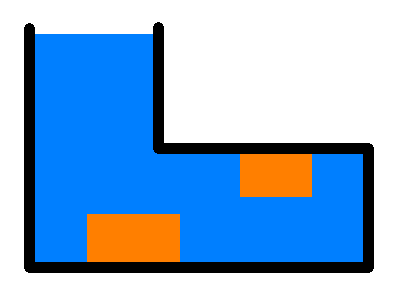
\includegraphics[width=1.3in]{figures/ap-blind-spot.png}
	\end{center}
	\caption{When Archimedes principle fails to hold.}
	\label{archimedes-principle-failing-case}
\end{figure}

Both of the two boxes have one of their surfaces sticking to the wall, but neither of the surfaces are overlapping the water's surface.
This means that if they are really touching the water, they should receive a non-zero pressure.
In these cases, formula (\ref{archimedes-principle-formula}) -- derived from the divergence theorem -- would be incorrectly taking the wall-surfaces' fake pressure into the sum of the net force, thus leading to a wrong result.

To deal with such case, we could explicitly calculate the original integral following formula (\ref{net-water-pressuring-force}) to get the correct result; but an immediate problem is that it would require us to actually integrate all the infinitesimals.
This is imposible for computers to achieve, so we need to transform them into finite surface fragments \cite{klosek1997integration}.

Most common 3D model formats are based on polygons, so this can be done with no difficulties.
The updated formula is given as (\ref{discretized-pressuring-force}).
\begin{equation}
	\mathbf{F}_P=\sum_{\text{face}}-\mathbf{n}\rho h|\text{face}|.
	\label{discretized-pressuring-force}
\end{equation}

Although this formula can be directly calculated by a computer, it leads to two new problems:
\begin{enumerate}
	\item It could be a huge performance cost to iterate through all surfaces of a mesh.
	\item After discretizing into non-infinitesimal surfaces, the simple-and-nice $\rho h$ for calculating the pressure doesn't hold anymore.
\end{enumerate}

The first problem is rather easy to see;
and the reason for the second problem is that, as though the position for an infinitesimal of the surface is clearly defined, a small surface fragment has its extend in the space.
Most commonly, a surface is not aligned directly to the Y-axis, and the different parts of it would be at different depth, resulting in experiencing different pressure (Figure \ref{water-pressure-differs-on-surface}).

\begin{figure}[h]
	\begin{center}
		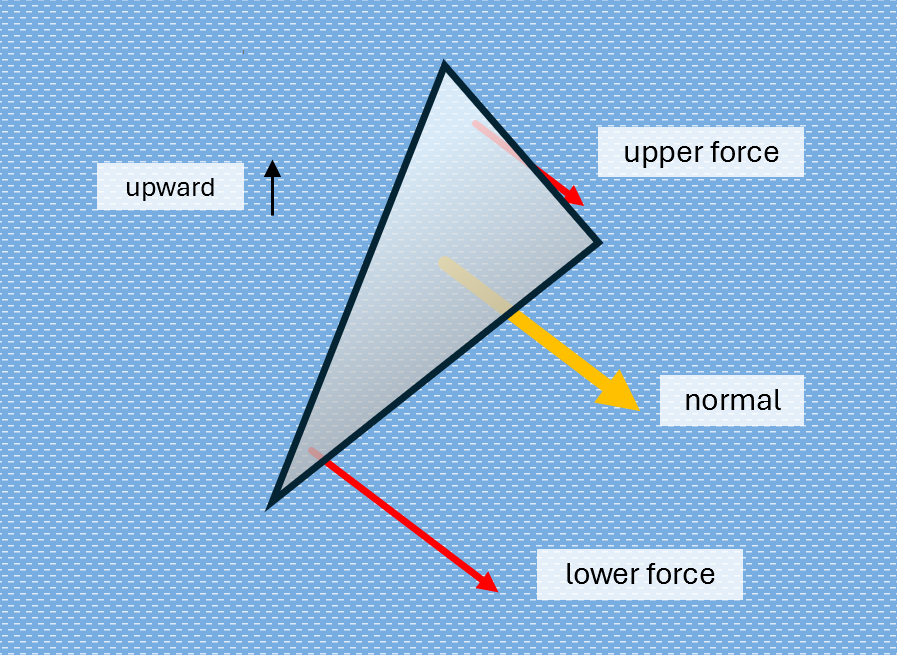
\includegraphics[width=3in]{figures/water-pressure-on-small-surface.png}
	\end{center}
	\caption{The water pressure differs on a surface.}
	\label{water-pressure-differs-on-surface}
\end{figure}